\documentclass[11pt,a4paper]{article}
\usepackage[T1]{fontenc}
\usepackage[margin=2.3cm]{geometry}
\usepackage{amsmath,amssymb}
\usepackage{graphicx}
\usepackage[dvipsnames]{xcolor}
\usepackage{enumitem}
\usepackage[colorlinks=true,linkcolor=blue,urlcolor=blue]{hyperref}
\setlength{\parskip}{0.6em}
\setlength{\parindent}{0pt}
\begin{document}

\begin{center}{\LARGE\bfseries openheartflow}\\[0.4em]{\large Build a pump and pipes model of the circulation and watch blood pressure appear.}\\[0.2em]\small PAN IIT OSS explainer \textbullet{} secondary school to diploma / undergraduate (levels 3-5)\end{center}

\section*{Why this exists}
Blood pressure is not a property of the blood alone: it comes from a pump pushing a fluid through pipes that resist and stretch. This explainer builds that idea in three steps, from flow = push / resistance, through Poiseuille's law, to the elastic-artery Windkessel model, using only numpy. It is general education, not medical advice, and the model is not a diagnostic tool.

\section*{The end goal}
Model blood circulation as a pump and pipes to see how blood pressure arises. The end goal is a pump and pipes model of the circulation that shows how blood pressure arises: why the small vessels dominate the resistance, why the pressure depends so strongly on vessel radius, and why stiffer arteries widen the pressure swing. The same mathematics appears in pipe networks, electrical circuits (an RC circuit) and shock absorbers.

\section*{How the three sessions build up}
\begin{enumerate}[nosep]
\item \textbf{Session 1: The heart is a pump, the vessels are pipes} (Level 1, conceptual interactive model, 60 min).
\item \textbf{Session 2: Resistance, cardiac output and mean pressure} (Level 2, mathematical engineering model, 75 min).
\item \textbf{Session 3: Elastic arteries: the two-element Windkessel model} (Level 3, simulation and validation, 90 min).
\end{enumerate}

\section{Session 1: The heart is a pump, the vessels are pipes}

\subsection*{A. Real-world problem}
Blood goes round and round in a closed loop of tubes; the same blood returns to the heart again and again. What pushes it, and why does the push have to be so much larger than it seems? Your heart is a pump, and the arteries, small vessels and veins are pipes that resist the flow. If the small vessels narrow, does the flow fall, or does the heart push harder? This is general education only: it is not medical advice and the model is not a diagnostic tool. Never use it to judge anyone's health.

\subsection*{B. Concept and theory}
A pump creates a pressure difference dP between the outlet and the return. The pipes resist the flow with a resistance R. The flow Q is dP divided by R: more push gives more flow, more resistance gives less flow. This is Ohm's law for pipes (voltage becomes pressure, current becomes flow). Pressure in medicine is quoted in mmHg (millimetres of mercury); flow of blood in litres per minute (L/min). The loop has three kinds of pipe one after another: the arteries, the small vessels (arterioles and capillaries, where blood feeds the tissues) and the veins. Pipes in a row add their resistances and the same flow passes through each, so the pressure lost in one pipe is Q times its resistance. The pressure therefore steps down along the loop and reaches the return pressure, which we take as 0. Typical textbook numbers: a push of 93 mmHg and a total resistance of 18.6 mmHg per L/min give 5 L/min. Our illustrative split of the resistance is 10 percent in the arteries, 80 percent in the small vessels and 10 percent in the veins.

\begin{itemize}[nosep]
\item dP: pressure difference produced by the pump (above the return pressure) (mmHg)
\item R: resistance of the pipes (mmHg per (L/min))
\item Q: flow of blood round the loop (L/min)
\item narrow: factor that multiplies the resistance of the small vessels (1 = normal) (no unit)
\end{itemize}

\begin{equation*}
Q=\frac{\Delta P}{R}
\end{equation*}

\begin{equation*}
R_{\mathrm{total}}=R_{\mathrm{arteries}}+R_{\mathrm{small}}+R_{\mathrm{veins}}
\end{equation*}

\begin{equation*}
\Delta P_{\mathrm{segment}}=Q\,R_{\mathrm{segment}}
\end{equation*}

\begin{center}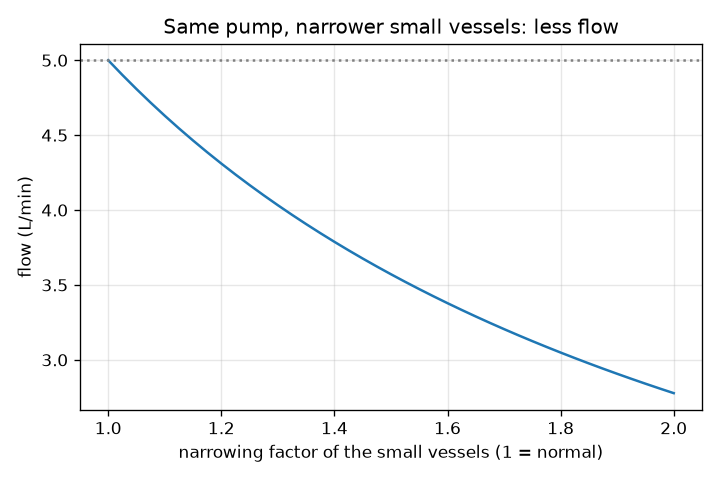
\includegraphics[width=0.85\linewidth]{figures/s01_flow_vs_narrowing.png}\\\small The same pump delivers less flow as the small vessels narrow.\end{center}

\subsection*{E. Worked example}
A pump gives 93 mmHg. The total resistance of the loop is 18.6 mmHg per L/min, split 10/80/10. Find the flow. Then the small vessels narrow so that their resistance is 1.5 times larger: find the new flow, and the push needed to keep 5 L/min.
\begin{enumerate}[nosep]
\item Total resistance = 0.10 x 18.6 + 0.80 x 18.6 + 0.10 x 18.6 = 18.6 mmHg per L/min.
\item Flow = 93 / 18.6 = 5.0 L/min. The small vessels lose 5.0 x 14.88 = 74.4 mmHg of the 93.
\item Narrowed: the small vessels now have 14.88 x 1.5 = 22.32; total = 1.86 + 22.32 + 1.86 = 26.04 mmHg per L/min.
\item Same pump: flow = 93 / 26.04 = 3.57 L/min.
\item To keep 5 L/min the pump must give 5 x 26.04 = 130.2 mmHg.
\end{enumerate}
\textbf{Answer.} Normal flow 5.0 L/min. After the narrowing the same pump gives 3.57 L/min; to restore 5 L/min the push must rise to 130.2 mmHg.

\subsection*{F. Questions}
\begin{enumerate}[nosep]
\item \textbf{Conceptual.} Why is the pressure highest at the heart outlet and lowest just before the heart, and why do the small vessels cause the largest drop?
\item \textbf{Numerical.} A pump gives only 60 mmHg through the typical resistance of 18.6 mmHg per L/min. What is the flow? Is the answer sensible?
\item \textbf{Graph and simulation interpretation.} In the pressure graph with narrowing 1.5 and a 93 mmHg pump, how much pressure do the small vessels use up, and how does that compare with normal vessels?
\item \textbf{Design and optimisation challenge.} Design: the pump can give at most 120 mmHg and the flow must stay at or above 4.5 L/min. How much can the small vessels narrow (to 2 decimal places)? State the trade-off.
\end{enumerate}

\section{Session 2: Resistance, cardiac output and mean pressure}

\subsection*{A. Real-world problem}
Your body can change the width of its small vessels in seconds, and a change of only a few percent in radius changes how hard the heart has to push. Why is the effect so large? If the resistance of the loop rises by 20 percent while the heart keeps pumping the same output, what happens to the pressure? And what would halving a vessel's radius do? All values are typical textbook figures, not a norm for any person; this is general education, not medical advice.

\subsection*{B. Concept and theory}
For slow, smooth (laminar) flow of a thick liquid of viscosity mu in a straight round tube of length L and radius r, Poiseuille's law gives the resistance R = 8 mu L / (pi r\textasciicircum{}4). The radius appears to the fourth power: the open area grows as r squared, and the average speed grows as r squared again, so the flow grows as r to the 4. Half the radius therefore gives 2\textasciicircum{}4 = 16 times the resistance. The heart ejects a stroke volume SV (mL) per beat; with heart rate HR (beats per minute) the cardiac output is CO = HR x SV, which is 70 x 70 mL = 4.9 L/min, about 5 L/min, for typical textbook values. The flow through the whole body obeys Q = dP / R, so with the return pressure taken as 0 the mean arterial pressure is MAP = CO x TPR, where TPR (total peripheral resistance) is the total resistance. Typical textbook values of 93 mmHg and 5 L/min give TPR = 18.6 mmHg per (L/min). From a reading 'systolic over diastolic' a common rule of thumb is MAP = diastolic + (systolic - diastolic)/3, which is 93.3 mmHg for 120/80.

\begin{itemize}[nosep]
\item mu: viscosity of blood (typical 3.5e-3, treated as constant) (Pa s)
\item L: length of the vessel (m)
\item r: radius of the vessel (m)
\item R: resistance of the vessel (Pa s / m\textasciicircum{}3 (or mmHg per mL/s))
\item HR: heart rate (beats per minute)
\item SV: stroke volume (blood pumped per beat) (mL)
\item CO: cardiac output (L/min)
\item TPR: total peripheral resistance (mmHg per (L/min))
\item MAP: mean arterial pressure (mmHg)
\end{itemize}

\begin{equation*}
R=\frac{8\,\mu\,L}{\pi\,r^{4}}
\end{equation*}

\begin{equation*}
\frac{R(r/2)}{R(r)}=2^{4}=16,\qquad \frac{R(kr)}{R(r)}=k^{-4}
\end{equation*}

\begin{equation*}
\mathrm{CO}=\mathrm{HR}\times\mathrm{SV}
\end{equation*}

\begin{equation*}
\mathrm{MAP}=\mathrm{CO}\times\mathrm{TPR}
\end{equation*}

\begin{equation*}
\mathrm{MAP}\approx P_{\mathrm{dia}}+\tfrac{1}{3}\,(P_{\mathrm{sys}}-P_{\mathrm{dia}})
\end{equation*}

\begin{center}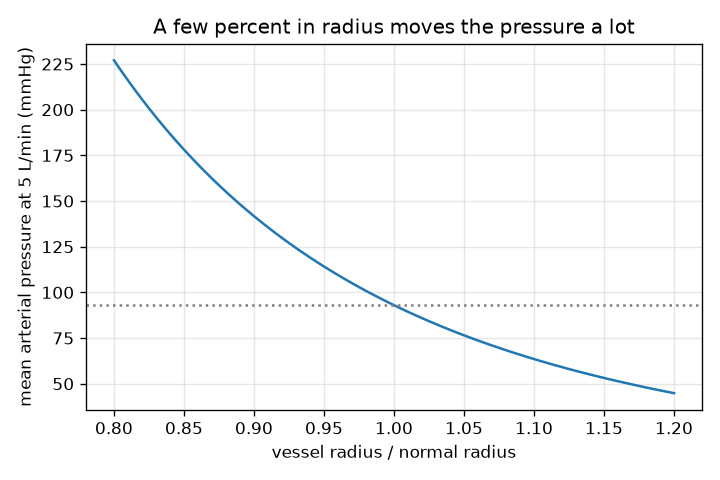
\includegraphics[width=0.85\linewidth]{figures/s02_map_vs_radius.png}\\\small MAP against vessel radius at 5 L/min: a few percent in radius moves the pressure a lot.\end{center}

\subsection*{E. Worked example}
A vessel 0.10 m long has radius 1.0 mm; blood has mu = 3.5e-3 Pa s. Find its resistance in mmHg per (mL/s), the flow for a push of 10 mmHg, and the same for radius 0.5 mm. Then: at a constant 5 L/min with TPR = 18.6, what happens to MAP if the resistance rises by 20 percent, and what radius change causes such a rise?
\begin{enumerate}[nosep]
\item R = 8 mu L / (pi r\textasciicircum{}4) = 8 x 3.5e-3 x 0.10 / (pi x (1.0e-3)\textasciicircum{}4) = 2.8e-3 / 3.142e-12 = 8.913e8 Pa s per m\textasciicircum{}3.
\item Convert: x 1e-6 (m\textasciicircum{}3 to mL) / 133.322 (Pa per mmHg) = 6.685 mmHg per (mL/s).
\item Flow for 10 mmHg: 10 / 6.685 = 1.496 mL/s.
\item Radius 0.5 mm: R is 16 times larger = 106.96 mmHg per (mL/s); the flow for 10 mmHg is 10 / 106.96 = 0.0935 mL/s, 16 times smaller.
\item TPR rises by 20 percent: 18.6 x 1.2 = 22.32. At constant 5 L/min, MAP = 5 x 22.32 = 111.6 mmHg (also 20 percent higher than 93).
\item The radius ratio k that gives resistance x1.2 satisfies k\textasciicircum{}-4 = 1.2, so k = 1.2\textasciicircum{}(-1/4) = 0.9554: the radius is only 4.5 percent smaller.
\end{enumerate}
\textbf{Answer.} R = 6.685 mmHg per (mL/s) for r = 1.0 mm and 106.96 for r = 0.5 mm (16 times). A 20 percent rise in resistance at constant output raises MAP from 93 to 111.6 mmHg, and it needs a radius only 4.5 percent smaller.

\subsection*{F. Questions}
\begin{enumerate}[nosep]
\item \textbf{Conceptual.} Why does the resistance depend on the radius to the fourth power and not just on the cross-section area (radius squared)?
\item \textbf{Numerical.} A heart beats 80 times per minute with a stroke volume of 60 mL. Find the cardiac output, and the MAP for a TPR of 18.6 mmHg per (L/min). Check the units.
\item \textbf{Graph and simulation interpretation.} In the graph of MAP against radius at 5 L/min, read the MAP at radius 0.9 and 1.1 of normal. Why are the two changes from 93 not equal?
\item \textbf{Design and optimisation challenge.} Design: the vessels are 5 percent narrower (radius 0.95 of normal) and the mean arterial pressure must stay at or below 100 mmHg. Find the largest cardiac output and choose a heart rate and stroke volume. State the trade-offs.
\end{enumerate}

\section{Session 3: Elastic arteries: the two-element Windkessel model}

\subsection*{A. Real-world problem}
The heart pushes blood out in short bursts, yet the pressure in the arteries never falls to zero between beats. Why? The big arteries are elastic: they swell during the burst, store blood, and squeeze it onwards while the heart rests, like the air chamber of an old fire pump (German: Windkessel). What sets the top and bottom pressure, and what happens when the arteries stiffen? This is general education; the model is a simplified illustration, not medical advice and not a diagnostic tool.

\subsection*{B. Concept and theory}
The arteries are modelled by two elements: an elastic compliance C (mL stored per mmHg of pressure rise) and a peripheral resistance R (mmHg s per mL) through which the stored blood drains. The ventricle forces in a flow Q\_in(t): a half sine during the first 0.3 of each beat (systole, the ejection) and zero afterwards (diastole). Its peak is chosen so that one beat delivers exactly the stroke volume SV. Blood stored in C grows with the inflow and drains through R, which gives C dP/dt = Q\_in(t) - P/R. In diastole Q\_in is zero and the exact solution is an exponential decay P = P0 exp(-t/(R C)) with time constant R C. Averaged over a periodic beat the stored blood does not change, so the mean pressure equals R times the mean inflow. We solve the equation with Runge-Kutta 4 (RK4): four slope estimates per step, error shrinking as the step to the 4th power. The pressure waveform has a systolic value (highest), a diastolic value (lowest) and a pulse pressure (their difference). Stiffer arteries mean a smaller C.

\begin{itemize}[nosep]
\item P: arterial pressure (the state of the model) (mmHg)
\item C: arterial compliance (mL / mmHg)
\item R: peripheral resistance (mmHg s / mL)
\item Q\_in: flow from the ventricle (mL/s)
\item SV: stroke volume (mL)
\item T\_s: duration of systole, 0.3 of the beat (s)
\item HR: heart rate (beats per minute)
\item tau = R C: time constant of the decay in diastole (s)
\end{itemize}

\begin{equation*}
C\,\frac{dP}{dt}=Q_{\mathrm{in}}(t)-\frac{P}{R}
\end{equation*}

\begin{equation*}
Q_{\mathrm{in}}(t)=\begin{cases}\dfrac{\pi\,SV}{2\,T_s}\sin\!\left(\dfrac{\pi t}{T_s}\right)&0\le t<T_s\\[2mm] 0&T_s\le t<T\end{cases}
\end{equation*}

\begin{equation*}
P(t)=P_0\,e^{-t/(RC)}\quad\text{(diastole)}
\end{equation*}

\begin{equation*}
\overline{P}=R\,\overline{Q}_{\mathrm{in}}=R\,\frac{SV\cdot HR}{60}
\end{equation*}

\begin{equation*}
y_{n+1}=y_n+\tfrac{\Delta t}{6}\,(k_1+2k_2+2k_3+k_4)
\end{equation*}

\begin{center}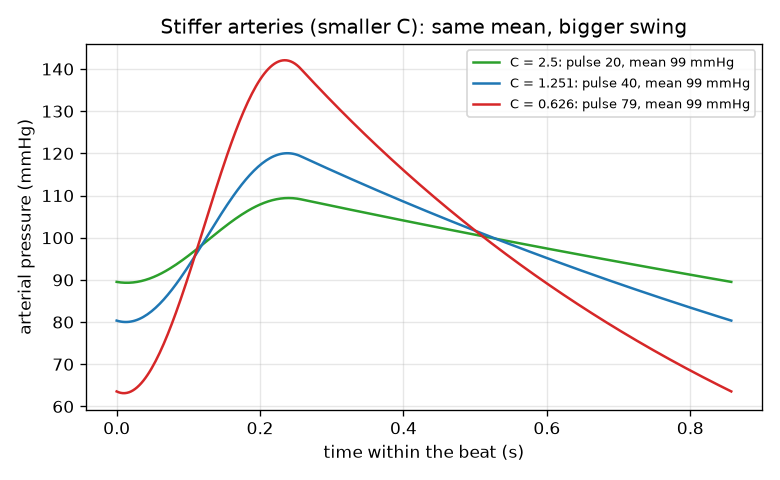
\includegraphics[width=0.85\linewidth]{figures/s03_stiffness_effect.png}\\\small Stiffer arteries (smaller C) give a larger pulse pressure at the same mean pressure.\end{center}

\subsection*{E. Worked example}
For R = 1.214 mmHg s/mL, C = 1.251 mL/mmHg, heart rate 70 and stroke volume 70 mL, find the time constant, the factor by which the pressure falls during diastole, the end-of-beat pressure when the pressure at the end of ejection is 119.3 mmHg, and the mean pressure from the mean-flow balance.
\begin{enumerate}[nosep]
\item Beat length T = 60/70 = 0.857 s; systole T\_s = 0.3 T = 0.257 s; diastole = 0.600 s.
\item Time constant tau = R C = 1.214 x 1.251 = 1.519 s.
\item Fall factor in diastole = exp(-0.600 / 1.519) = 0.674.
\item The simulation gives P = 119.3 mmHg at the end of ejection, so the pressure at the end of the beat is 119.3 x 0.674 = 80.4 mmHg.
\item The pressure dips to the minimum of 80.0 mmHg a hair after the next ejection starts (the inflow is still small), so the diastolic value is 80.0, the highest value is 120.0, and the pulse pressure is 40.0 mmHg.
\item Mean inflow = 70 x 70 / 60 = 81.67 mL/s, so the mean pressure = R x mean Q = 1.214 x 81.67 = 99.1 mmHg.
\end{enumerate}
\textbf{Answer.} tau = 1.519 s, fall factor 0.674, end-of-beat pressure 80.4 mmHg (minimum 80.0), pulse pressure 40.0 mmHg and mean pressure 99.1 mmHg (equal to the simulated mean).

\subsection*{F. Questions}
\begin{enumerate}[nosep]
\item \textbf{Conceptual.} Why does the arterial pressure not drop to zero in diastole when the heart is not pushing? Why does a stiffer artery change the pulse pressure but not the mean pressure?
\item \textbf{Numerical.} With R = 1.214, a heart rate of 60 beats per minute and a stroke volume of 70 mL, find the mean pressure from the mean-flow balance. Compare with the 70 beats case (99.1 mmHg).
\item \textbf{Graph and simulation interpretation.} In the stiffness figure the three waves have pulse pressures 20.1, 40.0 and 78.9 mmHg for C = 2.5, 1.251 and 0.626. What pattern do you see, and what is the mean pressure in each case?
\item \textbf{Design and optimisation challenge.} Design: choose R and C so that the model has a mean pressure of 90 mmHg and a pulse pressure close to 30 mmHg at 70 beats per minute and 70 mL. Report the systolic and diastolic values. This is an illustrative exercise, not a target for any person.
\end{enumerate}

\section{Real-world mini-project}
\textbf{Tune the arterial model to an illustrative 120/80 mmHg waveform.} Use \texttt{last\_beat} and \texttt{bp\_stats} from Session 3 with a heart rate of 70 beats per minute and a stroke volume of 70 mL. Find the peripheral resistance R and the compliance C for which the model's systolic pressure is 120 mmHg and its diastolic pressure is 80 mmHg, each within 1 mmHg. Hint: the mean-flow balance fixes the mean pressure from R, and the pulse pressure is mostly set by C, so adjust them in turn or use a two-variable Newton iteration with finite differences. The target 120/80 is a typical textbook figure used here as an illustration; it is not a norm for any person and the model must never be used to interpret anyone's blood pressure.

\section{The path ahead}
\begin{enumerate}[nosep]
\item \textbf{Session 4: A three-element Windkessel.} A model with a resistor in series with the compliance and resistance, solved with your own RK4.
\item \textbf{Session 5: Add a heart valve and let the stroke volume emerge.} A ventricle pressure model coupled to the Windkessel through a valve.
\item \textbf{Session 6: Arteries that stiffen with pressure.} A pressure-dependent compliance C(P) in the same RK4 solver.
\item \textbf{Session 7: A simple feedback on the resistance.} A controller that adjusts R each beat to hold the mean pressure at a set value.
\item \textbf{Session 8: From a lump to an arterial network.} A chain of Windkessel segments or a one-dimensional wave model.
\end{enumerate}

\section{Answers and hints}

\subsection*{Session 1}
\begin{enumerate}[nosep]
\item \textbf{Conceptual.} Hint: The pressure lost in a pipe is Q times its resistance, and the same Q flows through every pipe in a row. Solution: Blood flows from high to low pressure, and each pipe uses up pressure equal to Q times its resistance. The same flow Q passes every segment, so the segment with the largest resistance loses the most pressure. In our illustrative split the small vessels have 80 percent of the resistance, so they use up 80 percent of the push. The pressure reaches its lowest value (taken as 0) back at the heart.
\item \textbf{Numerical.} Hint: Q = dP / R. Solution: Q = 60 / 18.6 = 3.23 L/min. Sensible: a smaller push through the same pipes must give a smaller flow than the 5 L/min of the 93 mmHg case, and 60/93 of 5 is 3.2. Units: mmHg divided by mmHg per L/min is L/min.
\item \textbf{Graph and simulation interpretation.} Hint: Read the drop between the points at position 1 and position 2, or use Q times R of the small vessels. Solution: With narrowing 1.5 the flow is 3.57 L/min and the small vessels lose 3.57 x 22.32 = 79.7 mmHg (85.7 percent of the push), against 74.4 mmHg (80 percent) for normal vessels. The narrowed vessels take a bigger share of a smaller flow's pressure; the arteries and veins lose less, because the flow through them is smaller.
\item \textbf{Design and optimisation challenge.} Hint: The total resistance may be at most 120 / 4.5; solve 18.6 x (0.2 + 0.8 x narrow) for narrow. Solution: R\_total \textless{}= 120 / 4.5 = 26.67, so 0.2 + 0.8 x narrow \textless{}= 26.67 / 18.6 = 1.434, so narrow \textless{}= 1.54. At 1.54 the flow is 4.51 L/min; at 1.55 it is 4.48 L/min, just too low. Trade-off: a pump that must push this hard works much harder, and a real body cannot raise its pressure without limit. Assumptions: steady flow, the illustrative 10/80/10 split. General education only, not a clinical limit.
\end{enumerate}

\subsection*{Session 2}
\begin{enumerate}[nosep]
\item \textbf{Conceptual.} Hint: Flow = area x average speed. What happens to the average speed in a wider tube, where more of the liquid is far from the slow layer at the wall? Solution: The flow is the open area times the average speed. The area grows as r squared. In a wider tube more of the liquid is far from the wall, where friction slows it, so the average speed also grows as r squared for the same push. Together the flow grows as r\textasciicircum{}4, so the resistance shrinks as 1/r\textasciicircum{}4. The outcome: small changes in radius have a big effect.
\item \textbf{Numerical.} Hint: CO = HR x SV in mL per min, then divide by 1000. Solution: CO = 80 x 60 = 4800 mL/min = 4.8 L/min. MAP = 4.8 x 18.6 = 89.3 mmHg. Units: (L/min) x (mmHg per L/min) = mmHg. It is close to the typical 93 mmHg, as expected for a slightly lower output.
\item \textbf{Graph and simulation interpretation.} Hint: Evaluate 93 x r\textasciicircum{}-4 for both radii. Solution: At 0.9: 93 x 1.524 = 141.7 mmHg (a rise of 48.7). At 1.1: 93 x 0.683 = 63.5 mmHg (a fall of 29.5). The curve 1/r\textasciicircum{}4 is convex: narrowing raises the resistance faster than widening lowers it, so the two changes differ. Units: mmHg.
\item \textbf{Design and optimisation challenge.} Hint: TPR rises by 0.95\textasciicircum{}-4; then CO = MAP / TPR. Solution: The resistance factor is 0.95\textasciicircum{}-4 = 1.228, so TPR = 18.6 x 1.228 = 22.8. CO \textless{}= 100 / 22.8 = 4.38 L/min. For instance 60 beats per minute x 70 mL = 4.2 L/min gives MAP = 95.9 mmHg. Trade-off: a lower output delivers less blood to the tissues, so a real body would not simply choose this; the model has no regulation. Assumptions: constant viscosity, all small vessels narrowed together, typical textbook values. General education only.
\end{enumerate}

\subsection*{Session 3}
\begin{enumerate}[nosep]
\item \textbf{Conceptual.} Hint: Think of C as a store of blood and R as the tap that lets it out slowly. What does the mean-flow balance say the mean depends on? Solution: In diastole the stored blood drains through R, so the pressure decays exponentially with time constant R C, which is longer than the diastole, so it never reaches zero. A stiff artery stores less blood per mmHg (small C), so the same stroke volume makes a larger pressure swing: the pulse pressure grows. The mean pressure obeys mean P = R x mean Q, which contains neither C nor the shape of the wave, so it does not change.
\item \textbf{Numerical.} Hint: Mean inflow = SV x HR / 60 in mL/s, then multiply by R. Solution: Mean inflow = 70 x 60 / 60 = 70 mL/s, so mean P = 1.214 x 70 = 85.0 mmHg. It is lower than 99.1 by the factor 60/70, because the cardiac output is lower. Units: (mmHg s/mL) x (mL/s) = mmHg.
\item \textbf{Graph and simulation interpretation.} Hint: Compare C times pulse pressure for the three curves and look at the dotted mean lines. Solution: Halving C roughly doubles the pulse pressure (40.0 to 78.9, a factor 1.97): the pulse pressure is roughly inversely proportional to C, because the stroke volume must be stored in the compliance. The mean pressure is 99.1 mmHg in all three, as the mean-flow balance says. The wave of stiff arteries also reaches higher at the top (142.1) and lower at the bottom (63.2) around the same mean.
\item \textbf{Design and optimisation challenge.} Hint: R follows from the mean-flow balance; then try C values from 1.5 to 1.9 with last\_beat and bp\_stats. Solution: R = 90 / 81.67 = 1.102 mmHg s/mL. Trying C values: C = 1.7 gives systolic 105.3, diastolic 75.8, pulse pressure 29.5 mmHg and mean 90.0 mmHg, which is close to 30. A slightly smaller C would reach 30 exactly. Trade-off: the pulse pressure falls as C grows, but real arteries cannot be made arbitrarily soft, and the real mean pressure is also set by the whole body regulation, which the model does not include.
\end{enumerate}

\section{How to join}
Read \texttt{CONTRIBUTING.md} in the repository, then pick an issue labelled \texttt{good first issue}. Repository: \url{https://github.com/KrunalPanchal1995/openheartflow}

\end{document}
